\documentclass{article}

\usepackage[utf8]{inputenc}
\usepackage[spanish]{babel}
\usepackage{parskip}
\usepackage{graphicx}
\usepackage{fancyhdr}
\usepackage{hyperref}

\pagestyle{fancy}
\fancyhf{}

\setlength{\headheight}{14pt} 

\renewcommand{\headrulewidth}{0.5mm}

\fancyhead[R]{\uppercase{\leftmark}}
\fancyhead[L]{\textit{\nouppercase{\rightmark}}}
\fancyfoot[C]{\thepage}

\begin{document}

    
    \begin{titlepage}
        
        \centering
        
        
\includegraphics[width=0.8\textwidth]{imagenes/logo_UDP.png}\\[0.6cm]

        \textsc{\LARGE Universidad Diego Portales}\\[0.2cm]
        \textsc{\large Facultad de ingenieria y ciencias}\\[1.5cm]

        \rule{\linewidth}{0.5mm}\\[0.4cm]
        {\huge \bfseries Informe proyectos TIC's}\\[0.1cm]
        {\huge \bfseries V.I.A.}\\[0.1cm]
        {\huge \bfseries Visual Inteligence Assistant}\\[0.2cm]
        \rule{\linewidth}{0.5mm}\\[1.5cm]
        
        \textbf{Integrantes:} \\
        Camila Valencia \\
        Renato Riveros \\
        Cristobal \\
        Diego Valdés\\[0.6cm]

        \textbf{Profesor:}\\
        Nicolas Boetcher\\[0.6cm]

        \textsc{\large Viernes 17 de abril}

        \vfill

    \end{titlepage}

    \newpage
    \markboth{}{}
    \tableofcontents
    \newpage

    \section{Introducción}
    La entrada de la IA en la vida cotidiana sumada a la conectividad presente, abre la puerta al desarrollo de dispositivos inteligentes.

    Lamentablemente este potencial tecnologico esta centralizado, disponible casi en su totalidad para la población normativa, ignorando a ciertos grupos que forman parte de nuestra sociedad. Dirigir este desarrollo hacia herramientas
    que faciliten su forma de vivir disminuirá esta brecha latente.

    Este proyecto propone el desarrollo de un disposivo IoT de manos libres, enfocado en la asistencia y reconocimiento del entorno para las personas ciegas, llamado Visual Integence Assistant (V.I.A.) cuyo objetivo es aprovechar
    la tecnogia disponible, mejorando el entendimiento del entorno en estas personas.

    Para el desarrollo de este herramienta se creo el presente informe, que detalla el funcionamiento de la propuesta tecnologica, el estado del arte de las soluciones actuales disponibles, los posibles desafios tecnicos, ademas del plan necesario
    para la correcta implementación del dispositivo. 


    \newpage
    \section{Descripción del problema}
    Hoy gran parte de la autonomia de la personas ciegas y parcialmente videntes recae en su baston, este le entrega información a traves de sonidos y tacto sobre la superficie sobre la cual esta avanzando, otra herramienta util la tienen
    en su telefono personal, gracias a aplicaciones capaces de identificar etiquetas de alimentos, fechas de vencimiento o semaforos en la via publica. Ademas de la clasica videollamada con familiares o amigos para recibir ayuda al momento de comprar,
    esto en caso de que los mismos no esten presenetes fisicamente.

    Sin embargo, estas herramientas presentan algunas limitaciones, una de ellas es que son restrictivas entre si, es decir una persona ciega dificilmente puede estar analizando su entorno con el baston a la vez que sostiene un celular, lo que limita su
    capacidad de moverse adecuandamente.

    Por lo mencionado anteriormente surge la necesidad del desarrollo de un sistema que no comprometa su movilidad, que es ampliamente respaldada por su baston, esto da lugar a V.I.A. un dispositivo capaz de proporisonar el soporte visual que necesita, asi como la deteccion
    de objetos a traves de un sensor laser que busca complementar a la información recopilada por su baston.

    \newpage
    \section{Motivación}
    El proposito de V.I.A radica en la urgencia de abordar la carga emocional invisible que conlleva la discapacidad visual. Vivir en un entorno   diseñado por y para personas videntes genera una "burbuja de incertidumbre" constante, donde cada paso en un lugar desconocido se convierte en un ejercicio de tensión y duda. Nuestra principal motivación es disolver esa ansiedad, transformando el silencio del entorno en una voz amiga que no solo advierte sobre peligros a la altura de la cabeza o vehículos silenciosos, sino que devuelve al usuario la tranquilidad y la confianza para explorar el mundo sin miedo. \\

Más allá de la seguridad física, este proyecto nace del deseo de restaurar la espontaneidad y la dignidad en la vida cotidiana. Las herramientas tradicionales, aunque valiosas, a menudo limitan al usuario a una ruta rígida de supervivencia. Con VIA, buscamos que la tecnología actúe como un puente hacia la inclusión real, permitiendo que una persona pueda tomar decisiones informadas sin depender de la asistencia de terceros. Creemos firmemente que la autonomía es la base de la dignidad humana y que el progreso tecnológico carece de sentido si no se utiliza para nivelar el campo de juego para quienes enfrentan las mayores barreras. \\

Finalmente, como desarrolladores, nos mueve una convicción ética: el verdadero potencial de la Inteligencia Artificial debe medirse por su impacto social. En un mundo donde la innovación suele volcarse hacia el entretenimiento o la productividad corporativa, hemos decidido enfocar nuestro ingenio en un propósito humanista. V.I.A representa nuestro compromiso con la idea de que la visión no debería ser un privilegio, sino una experiencia compartida. No estamos construyendo solo un dispositivo electrónico; estamos diseñando una nueva forma de libertad que permite a las personas recuperar el control de su entorno y navegar la vida con la frente en alto.


    \newpage
    \section{objetivo}
    \subsection{Objetivo General}
El objetivo principal de este proyecto es diseñar y prototipar un dispositivo wearable de asistencia que utilice herramientas de visión artificial e Internet de las Cosas (IoT) para potenciar la autonomía de personas con discapacidad visual. Se busca crear un sistema que identifique elementos clave del entorno y posibles riesgos, entregando información útil al usuario de manera auditiva, permitiéndole navegar espacios públicos con mayor seguridad y confianza.

\subsection{Objetivos Específicos}
Para alcanzar esta meta, el proyecto se centra en la integración de hardware y software bajo un enfoque funcional. En primer lugar, se trabajará en la implementación de algoritmos de detección de objetos capaces de procesar imágenes capturadas por el dispositivo en tiempo real. La idea es que el sistema pueda reconocer patrones visuales básicos (como obstáculos a media altura o señales de tránsito) y convertirlos en alertas comprensibles, sin necesidad de que el usuario intervenga manualmente.

En cuanto al hardware, se busca mejorar el uso de sensores físicos y cámaras integradas en un marco ergonómico, priorizando que el procesamiento de la información se realice de forma eficiente dentro del mismo equipo. Un punto clave es la salida de información: se implementará un sistema de conducción ósea para que las descripciones del entorno lleguen al usuario de forma clara, pero sin bloquear sus oídos, permitiéndole mantener la atención auditiva en los sonidos naturales de la calle, lo cual es vital para su seguridad.

Finalmente, el dispositivo contará con capacidades de conectividad dentro del ecosistema IoT. El propósito de este módulo es permitir la sincronización de datos y la actualización de las funciones del asistente de manera remota. Al enfocarnos en la funcionalidad de la red como una herramienta de soporte para la actualización de información, buscamos que el dispositivo no sea un elemento aislado, sino un sistema capaz de evolucionar y adaptarse a las necesidades del usuario final a través de una conexión estable y sencilla.

    

    \newpage
    \section{Grupo y roles}
    A continuación se describen los roles de cada uno de los integrantes del equipo, estos roles se mantendrán a lo largo de la ejecución del proyecto. Los roles son los siguientes:

    \begin{itemize}
        \item\textbf{Desarrolador: Diego Valdés} será responsable de la programación y ensamblaje del controlador ESP-32 y sus sensores. En la fase actual del proyecto debe velar por la selección de los componentes.
        \item\textbf{Coordinador: Camila Valencia} Es responsable de la planificación de las tareas y la gestión general del equipo de trabajo. Velará por la buena comunicación entre el equipo.
        \item\textbf{Documentación: Cristobal gonzalez} estará enfocado en la documentación de la problematica asi como del codigo que se desarrolará, garantizando que esta facilite la escalabilidad de la solución.
        \item\textbf{Investigador: Renato Riveros} su responsabilidad será actuar como el puente entre el problema y la vialbilidad técnica del mismo, en esta fase inicial validará los datos oficiales y estudios, asegurando que la solución responda efectivamente a la problematica.
    \end{itemize}


    \newpage
    \section{Estado del arte}
    En el mercado actual se encuentran diversas soluciones para la asistencia de personas ciegas, estas se dividen es analogicas, biologicas y tecnologicas. A continuación se detallarán las mas relevantes de estas opciones.
    
        \subsection{Biologicas}:
            \textbf{Perros guias:} Una de las soluciones mas completas para este tipo de personas ya que avisa de obstaculos, localiza puertas, asientos, escaleras, entre otras cosas fundamentales para la navegación en lugares publicos y sirven de apollo emocional,
            el coste de entrega para el usuario es cero, sin embargo este debe correr con el alimento y gastos asociados al animal, sin embargo su coste de entrenamiento es alto y su disponibilidad baja.  Visitar perrosguia.cl

        \subsection{Analogicas}:
            \textbf{Baston:} el clasico que ha siempre ha acompañado a los ciegos, este los ayuda a identificar desniveles y objetos en su camino a traves del simple tacto.

        \subsection{Tecnologicas}:
            \textbf{OrCam MyEye:} Es un dispositivo que se acopla a los lentes del usuario, este se activa por comandos de voz y es capaz de trasmitir en forma de audio información visual en tiempo real y sin conección wifi. Braille Chile es su distribuidor oficial en el pais y nuevo tiene un coste de 7.5 millones de pesos iva incluido.
            La duración de su bateria esta limitida a 2 horas de uso, esto debido a su monitoreo continuo.

            \textbf{WeWalk Smart Cane:} Un bastón electrónico con sensores ultrasónicos para detectar obstáculos elevados y navegación GPS integrada. Su versión mas moderna, con asistencia de IA cuesta 1350 dolares segun su pagina oficial. Incluye 4 años de IA y de navegación guiada, estas funciones requieren conección a internet.

            \textbf{Lentes eSight:} Utilizados para potenciar la baja visión mediante pantallas internas de alta resolución. Su costo de adquisición es de 4.950 USD\@. Esta enfocado para personas con ceguera legal, es decir que, no es util para las personas con seguera total.

            \textbf{Seeing AI:} Es una aplicación gratuita altamente efectiva para reconocer textos, billetes y rostros. Su gran desventaja operativa es que obliga al usuario a sostener el celular con una mano, bloqueando un sentido táctil fundamental y exponiéndolo a riesgos de seguridad o caídas. Tambien requiere de una conección a internet.

            \textbf{Be My Eyes:} Conecta al usuario mediante videollamada con voluntarios videntes que pueden ayudar en tareas específicas como verificar la fecha de vencimiento de un alimento o leer una pantalla. Es costo cero pero requiere la voluntad de un tercero.

        Como se puede apreciar las alternativas tecnologicas disponibles se dividen en dos grupos, las que incluyen un dispositivo dedicado, manos libres, ofrecen grandes prestaciones pero poseen un alto costo, mientras que las aplicaciones moviles son gratuitas, aunque obligan al usuario a usar el telefono con sus manos, lo que limita su movilidad efectiva y puede ser un riesgo en la via publica.

        En este contexto, V.I.A se ubica como una de solución que sintetiza conceptos ya existentes, ya aprobadas por el mercado, en una solución manos libres a bajo costo que, espera mejorar la vida y autonomia de personas no videntes sin importat su status.

    \newpage
    \section{Tentativa de diseño}
    A continuación se describirá las propuestas conceptuales de como se deberia materializar V.I.A.

        \subsection{V.I.A. glasses}

            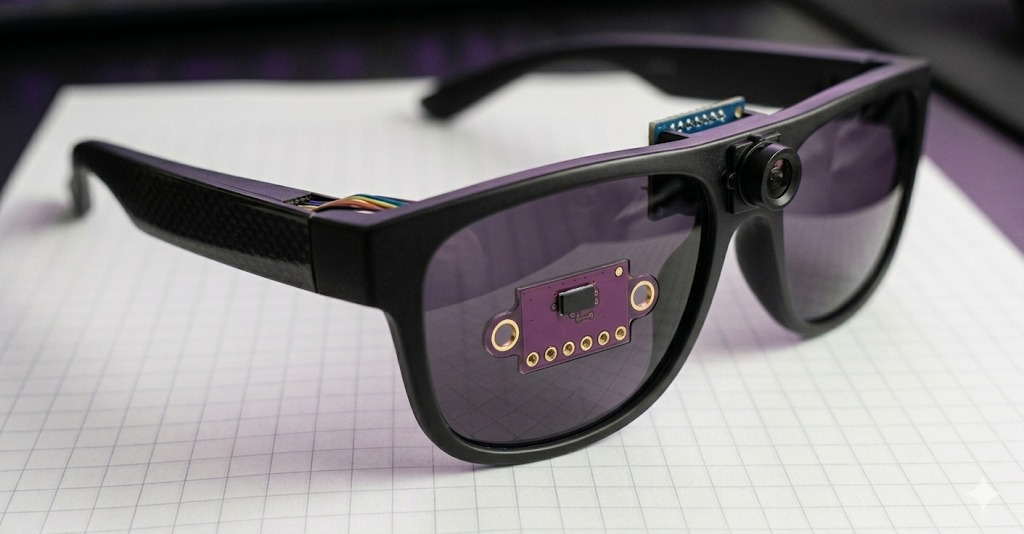
\includegraphics[width=0.6\textwidth]{imagenes/VIAglasses.jpeg}

            Como se puede apreciar en este arte conceptual ambos sensores irán la parte frontal de un lente, los cables de alimentación y de transmisión de datos viajarán a traves de una de las varillas del lente, estos cables estarán conectados a una especie de mochila que contiene al esp32 y a las baterias del mismo. Uno de los desafios de este modelo, es que la cantidad de cables necesarios para el modulo
            de la camara y puede incomodo para su usuario.

        \subsection{V.I.A. Beanie}
            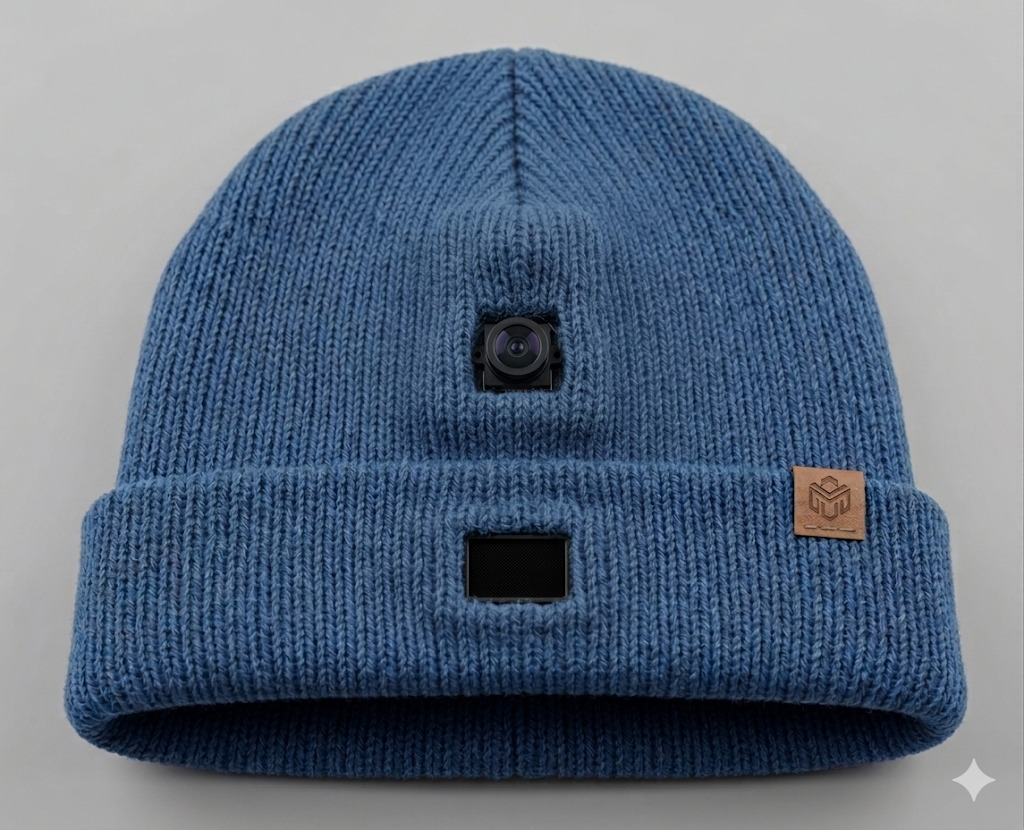
\includegraphics[width=0.6\textwidth]{imagenes/VIAbeanie.jpeg}

            Incorporar el controlador esp32 junto a ambos sensores y baterias en un solo gorro es posible, sin embargo este modelo poseé el incoveniente respecto a la posición de la camara, en su inclinación vertical como en su orientación frontal. 

    Durante el desarrollo de este proyecto de buscará dar soluciones a estas problematicas tecnicas.
    \newpage
    \section{Riegos}
    Para asegurar la viavilidad del proyecto, se han identificado areas que pueden representar desafios capaces de comprometer el correcto desarrollo, aqui se expondrán alguno riesgos y sus posibles soluciones.

        \subsection{Hardware:}El principal factor de riesgo en este ambito es la falla de los sensores, se intentará prevenir en la etapa de ensamblaje, soldando los componetes e implementado pruebas intensivas, tambien.

        \subsection{Software:}La latencia presente una gran problematica, por lo tanto esta prevista la compresión de la imagen, asi como un limite en los token que usará la IA por foto, limitando asi su respuesta y dismiyendo la latencia.

        \subsection{Usuario:}Por muy perfecto que sea el producto el usuario puede simplemente rechazarlo al no parecerle comodo, buscamos mitigar este problema a través de pruebas reales en etapas tempranas del proyecto. 
    \newpage
    \section{Plan de trabajo}
    El cronograma de nuestro proyecto se divide de forma general en 3 etapas en donde cada una consta de varias tareas ordenadas de una manera en que el tiempo de trabajo se aproveche al máximo teniendo plazos claros de entrega y mitigando el peligro de que exista algún retraso. A continuación se detallan las tareas y las etapas que se realizarán a lo largo del proyecto.

---

\subsection*{Abril: Inicio y presentación de ideas para el proyecto}

\begin{itemize}
    \item\textbf{Toma Requerimientos (1 de abril hasta 6 de abril):} Se realizan reuniones con fundaciones para tomar datos y consideraciones sobre el público al que queremos llegar.
    
    \item\textbf{Pruebas unitarias (6 de abril hasta 12 de abril):} Necesitamos saber qué tecnologías nos permite realizar y cumplir los requerimientos propuestos por lo que se hacen pruebas individuales a los elementos que vamos a usar (API, microcontrolador, módulos, sensores, etc).
    
    \item\textbf{Cotización y compras de componentes (6 de abril hasta 12 de abril):} Sabiendo lo que podemos y necesitamos realizar se compran el microcontrolador y sensores que utilizaremos.
    
    \item\textbf{Prototipo aplicación (12 de abril hasta 19 de abril):} Se presenta la idea de cómo se verá y cómo funcionará la aplicación que se creará.
    
    \item\textbf{Armado circuito electrónico (12 de abril hasta 19 de abril):} Se arma en una protoboard el circuito para conocer las conexiones que llevará y poder determinar qué tentativa de diseño vamos a utilizar.
    
    \item\textbf{Programación microcontrolador (26 de abril hasta 3 de mayo):} Se le asignan las funciones para procesar los datos de entrada de los sensores y determinar las acciones que debe realizar en base a estos.
    
    \item \textbf{Configuración de la API (26 de abril hasta 3 de mayo):} Una vez seleccionada la API se le dan las instrucciones para procesar la imagen y la base sobre lo que debe señalar además de asignarle una configuración para que sea más rápida la comunicación.
\end{itemize}

\subsection*{Mayo: Configuración y programación de software}

\begin{itemize}
    \item\textbf{Configuración text to speech (3 de mayo hasta 10 de mayo):} Se programa la función en donde el texto que devuelve la IA se transcribe a un audio y este es enviado al audífono para ser reproducido.
    
    \item\textbf{Programar aplicación (3 de mayo hasta 17 de mayo):} Se programará la aplicación móvil en donde esta tendrá principalmente las preferencias del usuario sobre la IA (estilo de voz, volumen, guardar consultas, etc).
    
    \item\textbf{Diseño prototipo físico (3 de mayo hasta 17 de mayo):} Se presentan ideas de cómo se vería todo físicamente ensamblado y así elegir el más cómodo y viable en términos de que la conexión no se interrumpa o no interrumpan al usuario.
    
    \item\textbf{Pruebas de flujo completo (10 de mayo hasta 17 de mayo):} Previo al ensamblado se prueba que todo el hardware y software funcione correctamente y no existan errores de conexión o comunicación entre dispositivos.
    
    \item\textbf{Ensamblar hardware (17 de mayo hasta 24 de mayo):} Una vez elegido el prototipo a utilizar y las pruebas de flujo estén completas con éxito se puede proceder a armar y montar todo.
    
    \item\textbf{Pruebas preliminares (24 de mayo hasta 31 de mayo):} Con el hardware ensamblado se empiezan las pruebas básicas para reconocer incomodidades o posibles problemas y/o errores y poder corregirlos.
\end{itemize}

\subsection*{Junio: Pruebas y pulir detalles}

\begin{itemize}
    \item\textbf{Pruebas de campo (1 de junio hasta 7 de junio):} La idea de esta tarea es poder facilitar un dispositivo a un usuario real y poder obtener un feedback conciso para después entregar una solución más completa.
    
    \item\textbf{Ajustes post feedback (7 de junio hasta 21 de junio):} Luego de obtener el feedback se realizan los ajustes necesarios satisfaciendo y resolviendo los problemas o sugerencias que nos dio el usuario.
    
    \item\textbf{Presentación final (29 de junio):} Ya resueltos todos los problemas del dispositivo y seguros que la solución y dispositivo presentado no tiene errores a nivel lógico y está bien diseñado a nivel físico lo presentamos en la feria de proyectos.
\end{itemize}

\vspace{1em}
\noindent Con este cronograma se tiene una visión clara de lo que se va a realizar dentro del plazo para completar el proyecto con metas y etapas específicas, esto entregar una solución robusta y completa hacia el público que queremos llegar y poder solucionar esta problemática que estamos abarcando.

\end{document}
